\begin{frame}
	\frametitle{Path Selection and Performance}
	\begin{itemize}
		\item Every conditional jump we must decide what path to follow first
		\begin{itemize}
			\item But some path may never terminate \\
			\only<2->{
				\centering\texttt{while ($3^{n}$ + $4^{n}$ == $5^{n}$) $\{$n++; ...$\}$}
			}
		\end{itemize}
		\item Exponential Blowup due to branches (running time, number of formulas and formula size)
	\end{itemize}
	\only<-2>{
		\centering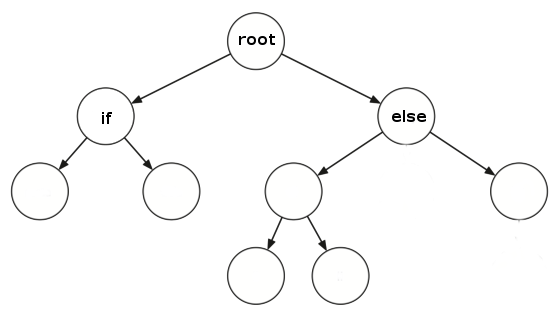
\includegraphics[scale=0.8]{tree}
	}
	\only<3->{
		\begin{itemize}
			\item Solutions
			\begin{itemize}
				\item \textbf{Path Selection Heuristic}
				\begin{itemize}
					\item Concolic Testing
					\item Depth-First or Random Search
				\end{itemize}
				\item More and faster \textbf{hardware}
				\item Identify \textbf{redundancies} between formulas or \textbf{independent subformulas}
			\end{itemize}
		\end{itemize}
	}
\end{frame}